\chapter{Техническое обслуживание}
%====================================================
% Техническое обслуживание
%====================================================

При техническом обслуживании отдельные исполнители выполняют следующие работы:
\begin{itemize}
    \item \textbf{механик-водитель}~--- мойку и чистку транспортера-тягача, подтяжку креплений и смазку агрегатов, узлов и механизмов, отдельные регулировки механизмов (совместно с механиком), перевод агрегатов на сезонные (зимние и летние) сорта горючего, смазки и охлаждающей жидкости, подготовку средств подогрева двигателя, обогрева, утепления и вентиляции;
    \item \textbf{механик}~--- проверку работы, регулировку и устранение неисправностей агрегатов и механизмов транспортера-тягача, промывку систем смазки и охлаждения двигателя, проверку работы на ходу после технического обслуживания и устранения замеченных недостатков; 
    \item \textbf{электрик}~--- проверку состояния электрооборудования и его крепление, устранение неисправностей в работе электрооборудования;  
    \item \textbf{слесарь}~--- подтяжку креплений агрегатов и механизмов, операции по смазке (совместно с механиком-водителем и его помощником). 
    
\end{itemize}

Для выполнения работ по ежедневному обслуживанию в помощь механику-водителю выделяются 1-2 чел. 

Операции по техническому обслуживанию транспортеров-тягачей выполняются с помощью индивидуальных (возимых) комплектов ЗИП и дополнительного инструмента и приспособлений, необходимых для работ по ТО-1 и ТО-2, входящих в комплекты Пункта технического обслуживания.

\section{Контрольный осмотр}

Контрольный осмотр~--- это совокупность операций, проводимых экипажем (механиком-водителем) в целях определения степени готовности объекта к применению по назначению. 

Цель контрольного осмотра (КО)~--- проверка технического состояния перед выполнением предстоящей задачи и устранение выявленных недостатков.

Контрольный осмотр является первичным видом контроля технического состояния.  Он проводится: 
\begin{itemize}
    \item при хранении объекта~--- ежемесячно;
    \item при использовании~--- перед выходом из парка, в пути (на привалах и длительных остановках), перед преодолением водной преграды и после ее преодоления. 
\end{itemize}

Продолжительность проведения контрольного осмотра:
\begin{itemize}
    \item перед выходом~--- \range{15}{20}~мин;
    \item на привалах~--- \range{10}{15}~мин.
\end{itemize}


\subsection{Содержание работ и технические условия перед выходом из парка}

\begin{figure}[]
    % // TODO нечитаемый текст на картинке
    \centering
    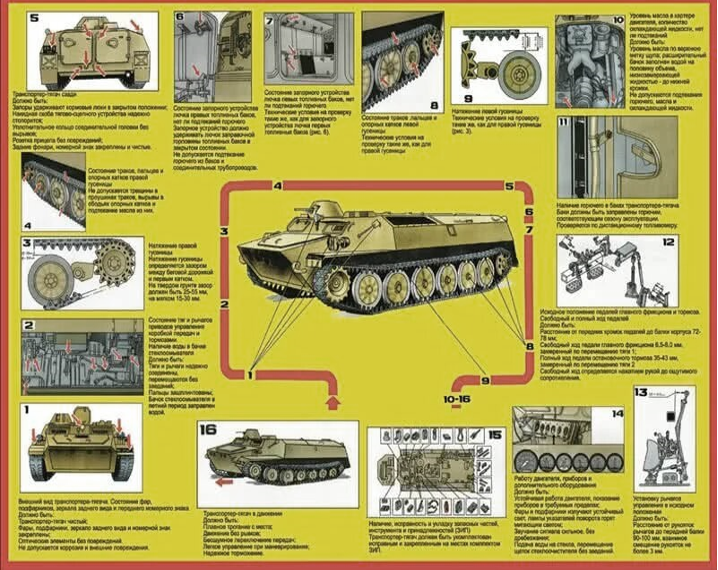
\includegraphics[width=\textwidth]{src/pic_1.png}
    \caption{Содержание работ и технические условия перед выходом из парка}
    \label{pic1}
\end{figure}


\subsubsection{По транспортеру-тягачу}

\begin{enumerate}
    \item Осмотреть транспортер-тягач, при необходимости удалить пыль, влагу, снег. 
    \item Установить аккумуляторные батареи, если они были сняты. 
    \item Проверить наличие и затяжку крышек люков в корпусе и на днище (после длительного перерыва в эксплуатации). 
\end{enumerate}

\subsubsection{По двигателю и его системам}

\begin{enumerate}
    \item Проверить: 
        \begin{itemize}
            \item уровень масла в картере двигателя (уровень масла должен быть по метке «В» на щупе); 
            \item уровень топлива в баках по топливомерной трубке, расположенной за сиденьем механика-водителя справа; 
            \item уровень охлаждающей жидкости (при заправке водой уровень должен быть до половины объема расширительного бачка, а при заправке низкозамерзающей жидкостью - по нижнюю кромку расширительного бачка); 
            \item нет ли подтекания охлаждающей жидкости, топлива или масла из радиаторов, баков, в местах соединений со шлангами, через сливные краники, в местах соединения трубопроводов и из фильтров (проверять после прогрева двигателя до температуры охлаждающей жидкости \celc{50}); обнаруженные подтекания устранить, а подтеки вытереть насухо; 
            \item уровень масла в топливном насосе и регуляторе, для чего вывернуть масляный щупг тщательно протереть его и установить во втулку до упора в резьбу. 
        \end{itemize}

    \item Пустить двигатель, на минимальных оборотах холостого хода (\range{450}{550}~об/мин) поработать \range{1}{2}~мин, увеличивая обороты, прогреть двигатель до температуры не ниже \celc{40}, прослушать его работу на разных оборотах коленчатого вала: дымления и посторонних шумов не должно быть.
    \item Проверить показания контрольно-измерительных приборов (масляных манометров системы смазки двигателя и главной передачи, манометра пневмосистемы и вольтамперметра). 
        
    \textbf{Показания должны быть:}
        \begin{itemize}
            \item давление масла в системе смазки двигателя на минимальных оборотах коленчатого вала не менее 1~кгс/см$^2$, при номинальных \range{4}{7}~кгс/см$^2$; 
            \item давление масла в главной передаче при эксплуатационных оборотах не менее 1,5~кгс/см$^2$; 
            \item давление воздуха в пневмосистеме \range{6}{7}~кгс/см$^2$; 
            \item величина зарядного тока (по амперметру) при номинальных оборотах коленчатого вала от 5 до 35~ампр. (в зависимости от заряженности аккумуляторных батарей). 
        \end{itemize}
\end{enumerate}


\subsubsection{По агрегатам, механизмам, системам}
\begin{enumerate}
    \item Проверить: 

\begin{itemize}
    \item исправность фар, приборов освещения и светосигнального устройства, звукового сигнала, сигнала «Стоп»; 
    \item исправность стеклоочистителя; 
    \item состояние и действие жалюзей радиатора; 
    \item нет ли утечки воздуха в пневмосистеме; 
    \item работу приводов управления и механизмов при переключении передач и поворотах транспортера-тягача (на ходу). 
\end{itemize}
\end{enumerate}


\subsubsection{По оборудованию и принадлежностям}
\begin{enumerate}
    \item Проверить:
    \begin{itemize}
        \item крепление шанцевого инструмента, ЗИП и огнетушителей; 
        \item состояние тягово-сцепного прибора; 
        \item плотность соединения соединительной головки со шлангом тормозной системы прицепа при полностью открытом разобщительном кране (при эксплуатации без прицепа кран должен быть закрыт). 
    \end{itemize}
\end{enumerate}

\subsubsection{Дополнительные работы, проводимые при эксплуатации зимой и в районах Крайнего Севера}

\begin{enumerate}
    \item Поставить аккумуляторные батареи. 
    \item Перед прогревом двигателя проверить, не застыла ли низкозамерзающая жидкость. Подогревать двигатель в строгом соответствии с заводской инструкцией. 
    \item При температуре воздуха ниже минус \celc{25} в главной передаче, бортовых передачах, ступицах опорных катков и направляющих колес применять масло МТ-14п. 
    \item Перед маршем по снежной целине и безлесной местности проверить исправность приспособлений для самовытаскивания и буксирных приспособлений. 
    \item Уложить бревно на транспортер-тягач. 
\end{enumerate}

\subsubsection{Дополнительные работы, проводимые при эксплуатации в горных районах:}

\begin{enumerate}
    \item Проверить наличие и исправность горных приспособлений (дополнительные грунтозацепы и др.). 
\end{enumerate}



\subsection{Содержание работ и технические условия в пути (на привалах и остановках)}
\subsubsection{По двигателю и его системам}
\begin{enumerate}
    \item Проверить: 
        \begin{itemize}
            \item уровень масла в картере двигателя, топлива в баках и охлаждающей жидкости в расширительном бачке; при необходимости дозаправить; 
            \item нет ли подтеканий охлаждающей жидкости, топлива, масла; обнаруженную течь устранить, а вытекшую смазку вытереть насухо. 
        \end{itemize}
\end{enumerate}

\subsubsection{По силовой передаче, ходовой части и механизмам управления}
\begin{enumerate}
    \item Проверить: 
    \begin{itemize}
        \item нагрев картеров бортовых передач, ступиц направляющих колес и опорных катков; нагрев считается нормальным, если не вызывает ощущения ожога ладони руки; 
        \item состояние траков и пальцев гусеничных цепей; траки, имеющие трещины, опасные для дальнейшей работы, и поломанные пальцы должны быть заменены; 
        \item натяжение гусеничных цепей; при необходимости отрегулировать, их натяжение (см. технологическую карту №\ref{techcard25}). 
    \end{itemize}
\end{enumerate}


\subsubsection{По оборудованию и принадлежностям}
\begin{enumerate}
    \item Проверить: 
    \begin{itemize}
        \item надежность сцепки с прицепом, исправность тягово-сцепного прибора и плотность соединения соединительной головки со шлангом тормозной системы; 
        \item состояние и крепление груза в кузове и на прицепе; 
        \item крепление ЗИП, шанцевого инструмента и огнетушителей; 
        \item состояние ходовой части прицепа. 
    \end{itemize}
\end{enumerate}

\subsubsection{Дополнительные работы, проводимые при эксплуатации зимой и в районах Крайнего Севера}
\begin{enumerate}
    \item Во время стоянки транспортера-тягача и особенно при сильном морозе периодически пускать и прогревать двигатель. 
    \item Сбить снег или лед, намерзший на беговых дорожках гусениц. 

\end{enumerate}



\section{Ежедневное техническое обслуживание}
Ежедневное техническое обслуживание (ЕТО) проводится с целью контроля исправного состояния машины, обеспечивающего безопасность движения, а также заправки топливом, маслом и охлаждающей жидкостью и поддержания внешнего вида, а также обеспечении последующей надежной работы при пробеге не менее \range{250}{300}~км. Ежедневное техническое обслуживание проводится экипажами (механиками-водителями) с участием специалистов подразделений технического обеспечения в конце дня после каждого выхода из парка независимо от пробега (в конце суток боевых действий).

Ежедневное техническое обслуживание включает:
\begin{itemize}
    \item общий контроль технического состояния машины; 
    \item дозаправку ГСМ, боеприпасами (во время боевых действий);
    \item мойку (чистку);
    \item проверку комплектности.
\end{itemize}

Последовательность выполнения работ ежедневного технического обслуживания определяется командиром в соответствии с условиями проведения работ, наличием экипажа и имеющимся временем. 

В первую очередь выполняются работы, которые влияют на боеготовность образцов ВВТ (пополнение боеприпасов, дозаправка ГСМ и т.д.). 

В парке работы ежедневного технического обслуживания производятся в технологической последовательности прохождения машины по элементам линии технического обслуживания.

Продолжительность проведения ежедневного технического обслуживание определяется приказом МО 1998~г. и действующими инструкциями по техническому обслуживанию и составляет: \range{1,5}{2} часов.


\subsection{Содержание работ и технические условия}
\subsubsection{По транспортеру-тягачу}
\begin{enumerate}
    \item Сразу после пробега (при наличии в раме топлива, масла и воды) поставить транспортер-тягач на уклон с креном на корму или нос, открыть кингстоны для слива скопившегося топлива, масла, воды. 
    \item Осмотреть нет ли подтекания масла из агрегатов силовой передачи и ходовой части и проверить степень их нагрева. 
    \item Заправить транспортер-тягач топливом. 
    \item Проверить уровень масла и охлаждающей жидкости и при необходимости дозаправить. 
    \item Очистить и вымыть транспортер-тягач снаружи, убрать в кабине и кузове, вытереть насухо все узлы, стекла кабины, фар, прожектора, задних фонарей и мастику аккумуляторных батарей; протереть днище рамы и закрыть кингстоны.
    \item Проверить состояние днища (нет ли деформаций и пробоин), наличие и затяжку крышек люков. 
    \item Устранить неисправности, обнаруженные в пути и при обслуживании. 
\end{enumerate}

\subsubsection{По двигателю и его системам}
\begin{enumerate}
\item Проверить не подтекает ли охлаждающая жидкость из радиатора в местах соединений со шлангами и из сливных краников; не подтекает ли топливо и масло в местах соединений трубопроводов, из фильтров. Обнаруженные подтекания устранить, а подтеки вытереть насухо. 
\item Спустить 0,1~л топлива из фильтров грубой очистки и тонкой очистки. После этого дать двигателю поработать \range{3}{4}~мин для удаления воздушных пробок.
\item Проверить состояние и натяжение ремней приводов генератора, водяного насоса, компрессора и вентилятора. При необходимости отрегулировать (см. технологические карты №\ref{techcard8}, \ref{techcard9}, \ref{techcard10} и \ref{techcard11}). 

\textbf{При нажатии большим пальцем руки с усилием \range{3}{4}~кгс прогиб должен быть, \textit{мм}:}
\begin{itemize}
    \item на короткой ветви ремней привода генератора \range{10}{12}; 
    \item на середине ветви ремня привода водяного насоса \range{10}{15}; 
    \item на середине ветви ремня привода компрессора \range{5}{8};
    \item на верхней ветви ремней привода вентилятора \range{8}{14}. 
\end{itemize}

\item Проверить уровень масла в регуляторе числа оборотов и в топливном насосе. Уровень масла должен быть по верхнюю метку на щупе. При необходимости дозаправить. 
\end{enumerate}


\subsubsection{По электрооборудованию}
\begin{enumerate}
    \item Проверить крепление и, работу фар, поворотной фары-искателя, задних фонарей и звукового сигнала, включив выключатель массы. Ослабление крепежных деталей не допускается. 
    \item Через каждые 15 дней, а в жаркое время через \range{5}{6} дней, проверить уровень и плотность электролита в батареях, крепление аккумуляторных батарей и прочистить вентиляционные отверстия в них. Через каждые \range{30}{35} дней независимо от степени заряженности аккумуляторные, батареи заряжать на зарядной станции. Уровень электролита должен быть выше предохранительного щитка на \range{8}{10}~мм. 
\end{enumerate}



\begin{sidewaystable}
    \center
    \begin{tabular}{|m{5cm}|m{1.5cm}|>{\tc}m{4.5cm}|>{\tc}m{4.5cm}|}
        \hline
        \multicolumn{2}{|m{6.5cm}|}{\tc Районы эксплуатации} & Минимальная окружающая температура, \celc{} & Плотность электролита заряженных батарей при~его температуре $+$\celc{15} \\
        \hline
        \multicolumn{2}{|m{6.5cm}|}{\tc Южные} & до $-$20 & 1,25 \\
        \hline
        \multicolumn{2}{|m{6.5cm}|}{\tc Центральные} & до $-$30 & 1,27 \\
        \hline
        \multicolumn{2}{|m{6.5cm}|}{\tc Северные} & до $-$40 & 1,29 \\
        \hline
        \multirow{2}{5cm}{\tc С резко континентальным климатом} & \tc зимой && 1,31 \\
        \cline{2-4}
        & \tc летом & & 1,27 \\
        \hline
    \end{tabular}

    \caption{Плотность электролита полностью заряженных батарей для различных климатических условий эксплуатации}
    \label{electrolyte_density}

    \flushleft
    \textit{Примечания:}
    \begin{itemize}
        \itshape
        \item Степень разряженности батарей при эксплуатации зимой допускается не более 25~\%, а~летом~--- не более 50~\%.
        \item Понижение плотности электролита на 0,01 соответствует разрядке батареи примерно на \range{5}{6,25}~\%.
    \end{itemize}
\end{sidewaystable}

\newpage

\subsubsection{По силовой передаче, ходовой части и механизмам управления}
\begin{enumerate}
    \item Провернуть на \range{два}{три} оборота рукоятку оси масляного фильтра главной передачи. 
    \item Проверить: 
    \begin{itemize}
        \item состояние торсионов, траков и пальцев гусениц; 
        \item натяжение гусениц; правильность натяжения определяется по положению верхней ветви. Она должна лежать на четырех опорных катках, не касаясь первого и шестого катков. При необходимости отрегулировать (см. технологическую карту №\ref{techcard25}); 
        \item состояние резиновых бандажей опорных катков;
        \item крепление гидравлических амортизаторов; 
        \item нет ли утечки воздуха из пневмосистемы. 
    \end{itemize}
\end{enumerate}


\subsubsection{По оборудованию и принадлежностям}
\begin{enumerate}
    \item После возвращения из рейса, открыть кран отбора воздуха и слить конденсат из баллонов пневмосистемы. 
    \item Проверить: 
    \begin{itemize}
        \item состояние и крепление тягово-сцепного прибора; 
        \item состояние вооружения (в соответствии с наставлением по вооружению) и укладку боеприпасов (МТЛБ); 
        \item состояние смотровых приборов (МТЛБ) и при необходимости очистить их; 
        \item укладку и крепление ЗИП; 
        \item крепление огнетушителей. 
    \end{itemize}
\end{enumerate}


\subsubsection{По смазке}
\begin{enumerate}
    \item Смазать агрегаты и механизмы транспортера-тягача согласно таблице смазки.
\end{enumerate}

\begin{figure}[h]
    \centering
    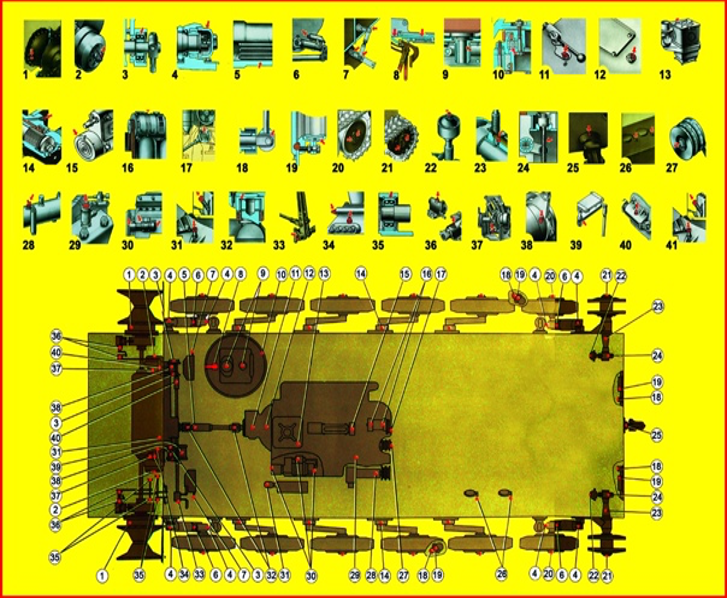
\includegraphics[width=\textwidth]{src/lubricant.png}
    \caption{Схема смазки}
    \label{lubricant}
\end{figure}


\subsubsection{Дополнительные работы, проводимые при эксплуатации зимой и в районах Крайнего Севера}
\begin{enumerate}
    \item Если предвидится длительный перерыв в эксплуатации транспортера-тягача при хранении его на открытом воздухе или в неотапливаемом помещении при температуре наружного воздуха ниже минус \celc{15}, снять аккумуляторные батареи и поставить их в отапливаемое помещение. 
    \item Проверить исправность средств подогрева. 
    \item Открыть нижнюю пробку камеры горения отопительно-вентиляционной установкой. ОВ-65 и слить конденсат. 
    \item Проверить, нет ли воды во впускных и выпускных патрубках. 
\end{enumerate}

\subsubsection{Дополнительные работы, проводимые при эксплуатации в районах песчано-пустынной и на сильно запыленной местности}
\begin{enumerate}
    \item Очистить поверхность радиатора от песка и пыли. 
    \item Через \range{4}{5} дней проверить работу паровоздушного клапана пробки расширительного бачка. 
    \item Через \range{25}{30}~ч работы двигателя очистить и промыть фильтрующий элемент, бункер и циклоны воздухоочистителя (см. технологическую карту №\ref{techcard7}).
    \item Очистить и промыть атмосферные фильтры в пробках заливных 
горловин. 
\end{enumerate}

\subsubsection{Дополнительные работы, проводимые при эксплуатации в горных районах}
\begin{enumerate}
    \item Если ожидается понижение температуры воздуха ниже нуля, слить воду из системы охлаждения (чтобы меньше было накипи эту же воду целесообразно вновь использовать для заправки системы охлаждения). 
    \item Один раз в три дня проверять уровень электролита в батареях.
\end{enumerate}

\subsubsection{Дополнительные работы, проводимые после преодоления бродов (водных преград)}
\begin{enumerate}
    \item Смазать подшипники механизма выключения фрикционов механизмов поворота. 
    \item Проверить наличие воды, в масле бортовых передач, главной передаче, опорных катков и направляющих колес. При обнаружении следов воды (масло имеет серый цвет, повышенный уровень масла, наличие воздушных пузырьков) масло заменить. 
    \item При необходимости промыть систему водооткачивания заливкой воды через водовыбрасывающий патрубок, слив воды -  через кингстоны, не включая водооткачивающий насос. 
\end{enumerate}

\subsubsection{Дополнительные работы, проводимые при эксплуатации в условиях грязных дорог и распутицы}
\begin{enumerate}
    \item По окончании периода интенсивной ежедневной эксплуатации, но не более чем через 500 км пробега, проверить уровень масла в картерах бортовых передач и при обнаружении воды или грязи в масле, сменить его. 
    \item В случае повышенного нагрева охлаждающей жидкости системы охлаждения двигателя - снять жалюзи, очистить и промыть водой поверхность радиатора от грязи.

\end{enumerate}


\section{Техническое обслуживание №1}
Техническое обслуживание №1 (ТО-1) предназначено для детальной проверки технического состояния машины, выявления и устранения неисправностей, обеспечения безотказной работы машины до очередного номерного обслуживания.

Техническое обслуживание №1 выполняется в пункте технического обслуживания и ремонта (ПТОР) для гусеничных тягачей и транспортеров~--- через \range{800}{1000}~км. 

Техническое обслуживание №1 включает объем ЕТО и ряд дополнительных операций по контрольной диагностике, смазке, проверке крепления, исправности и укомплектованности механизмов и агрегатов, выполнения необходимых регулировок и устранению обнаруженных неисправностей. Они в основном выполняются без разборки агрегатов.

Техническое обслуживание №1 проводится личным составом, закрепленным за вооружением и техникой, с привлечением сил и средств технического обеспечения соединения (части, подразделения). Организует командир подразделения.

Средняя трудоемкость технического обслуживания №1 (без учета уборочно-моечных работ) для гусеничных машин составляет 10 чел./час. Простой машин на техническом обслуживании №1 для гусеничных машин~--- 6 часов. 

\subsection{Содержание работ и технические условия}
Выполнить все операции, указанные для ежедневного технического обслуживания. Дополнительно провести следующие работы: 


\subsubsection{По двигателю и его системам}
\begin{enumerate}
    \item Проверить крепление: 
    \begin{itemize}
        \item опор двигателя
        \item топливных баков
        \item натяжного ролиБрезент должен быть закреплен так, чтобы он не соприкасался с землей, не раздувался ветром; на поверхности брезента нежка 
        \item масляного и водяного насосов
        \item топливного насоса высокого давления
        \item радиатора
        \item других приборов систем питания, смазки, охлаждения.
    \end{itemize}
    Ослабление креплений не допускается. При необходимости подтянуть.
    
    \item Проверить:
        \begin{itemize}
            \item состояние и герметичность трубопроводов, агрегатов и приборов систем смазки, питания и охлаждения; при необходимости неисправности устранить: 
            \item регулировку привода управления топливным насосом; 
            \item работу механизма останова двигателя; 
            \item состояние паровоздушного клапана расширительного бачка (загрязнение и легкость хода штока клапана); в случае заедания промыть клапан горячей водой; 
            \item плотность низкозамерзающей жидкости (в зимнее время). 
            
            \textbf{Плотность жидкости «40» должна быть \range{1,068}{1,073}, а жидкости «65»~--- \range{1,085}{1,090}.}
        \end{itemize} 
    \item Промыть фильтр центробежной очистки масла (см. технологическую карту №\ref{techcard5}). 
    \item Промыть фильтр грубой очистки масла (через одно ТО-1), (см.  технологическую карту №\ref{techcard4}), очистить и промыть через 50 ч работы двигателя фильтрующий элемент, бункер и циклоны воздухоочистителя (см. технологическую карту №\ref{techcard7}). 
    \item При работе в пыльных условиях очистить сердцевину радиатора системы охлаждения от пыли и грязи. Промыть и продуть сжатым воздухом сапун топливного насоса высокого давления. 
\end{enumerate}

\subsubsection{По электрооборудованию}
\begin{enumerate}
    \item Проверить и при необходимости очистить зажимы аккумуляторных батарей от окиси, затянуть и слегка смазать, 
    \item Проверить: 
    \begin{itemize}
        \item крепление генератора, стартера, реле-регулятора и при необходимости подтянуть; 
        \item состояние всех контактов электроприборов, при необходимости зачистить и затянуть крепления. 
    \end{itemize}
\end{enumerate}

\subsubsection{По силовой передаче и ходовой части}
\begin{enumerate}
    \item Проверить: 
        \begin{itemize}
            \item крепление венцов ведущих колес, карданного вала промежуточного редуктора, гаек балансиров, колпаков опорных катков, направляющих и ведущих колес, корончатых гаек коленчатых осей и ободьев направляющих колес, конических пружин упоров, приспособлений для снегоочистителя, механизмов и приводов управления транспортера-тягача, при необходимости подтянуть крепления и зашплинтовать; 
            \item крепление тормозного крана и пневмокамер тормозов, открыв люк главной передачи. 
            \item регулировку механизмов поворота и остановочных тормозов, при необходимости отрегулировать (см. технологические карты №\ref{techcard23} и \ref{techcard19}); 
            \item исправность предохранительного клапана пневмосистемы; при повышении давления больше 7,5 кгс/см$^2$ клапан снять, промыть и отрегулировать; 
            \item шплинтовку шарнирных соединений приводов управления транспортера-тягача. 
        \end{itemize}
    \item Слить отстой из масляного фильтра главной передачи (сразу после возвращения из рейса в парк). 
    \item Проверить и при необходимости отрегулировать полный и свободный ход педали главного фрикциона (см. технологическую карту №\ref{techcard18}).
\end{enumerate}

\subsubsection{По оборудованию и принадлежностям}
\begin{enumerate}
    \item Проверить состояние огнетушителей путем взвешивания, при необходимости подзарядить (минимально допустимый вес заряда огнетушителей ОУ-2 1,25 кг). 
    \item Проверить герметичность корпуса.
\end{enumerate}

\subsubsection{По агрегатам и механизмам}
\begin{enumerate}
    \item Проверить работу механизмов управления при переключении передач и на поворотах (на ходу транспортера-тягача); при необходимости отрегулировать их (см. технологические карты №\ref{techcard19}, \ref{techcard20}, \ref{techcard21}, \ref{techcard22}, \ref{techcard23} и \ref{techcard24}). 
\end{enumerate}

\subsubsection{По смазке}
\begin{enumerate}
    \item Смазать агрегаты и механизмы транспортера-тягача согласно таблице смазки.
\end{enumerate}

\subsubsection{Дополнительные работы, проводимые при эксплуатации в песчано-пустынных районах и на сильно запыленной местности}
\begin{enumerate}
    \item Очистить и смазать посадочные места коленчатых осей направляющих колес и гнезда кронштейнов (при затрудненном проворачивании коленчатых осей). 
    \item После 25-30 ч работы двигателя очистить фильтрующие элементы воздухоочистителя (промыть в дизельном топливе) от пыли, грязи и промаслить фильтрующие элементы в масле МТ-16п, смазать войлочные уплотнители и прокладки.
\end{enumerate}


\section{Техническое обслуживание №2}
Техническое обслуживание №2 (ТО-2) предназначено для обеспечения безотказной работы агрегатов, узлов и систем машины в пределах установленных норм, снижения интенсивности износа деталей, выявления и предупреждения отказов и неисправностей путем своевременного проведения контрольно-диагностических, смазочных, крепежных, регулировочных и других работ.

Техническое обслуживание №2  выполняется также в ПТОР для гусеничных тягачей и транспортеров через \range{2400}{3000}~км,

Техническое обслуживание №2  включает объем работ, технического обслуживания №1 и, кроме того, установленные нормативно-технической (эксплуатационной) документацией дополнительные операции, для выполнения которых требуется частичная или полная разборка отдельных агрегатов, узлов и аппаратуры с заменой сборочных единиц, отработавших или отслуживших установленный ресурс и не соответствующих требуемым пара¬метрам.

Этим обслуживанием завершается цикл технического обслуживания машины.

Техническое обслуживание №2  выполняется специалистами ПТОР при участии механика-водителя обслуживаемой машины.

Средняя трудоемкость технического обслуживания №2  составляет: для гусеничных машин соответственно 13 и 25 чел./час. Простой машин при техническом обслуживании №2  планируется из расчета-гусеничных машин~--- 12 ч.

Исполнители~--- механик, механик-водитель, электрик и слесарь. 

\subsection{Содержание работ и технические условия}
Выполнить все операции, указанные для технического обслуживания №1. Дополнительно провести следующие работы:

\subsubsection{По двигателю и его системам}
\begin{enumerate}
    \item Проверить: 
        \begin{itemize}
            \item угол опережения впрыска топлива, при необходимости (через одно ТО-2) отрегулировать (см. технологическую карту №\ref{techcard13}); 
            \item зазоры клапанного механизма, при необходимости отрегулировать; (зазоры у впускного и выпускного клапанов должны быть \range{0,25}{0,30}~мм, см.~технологическую карту №12); 
            \item положение педали подачи топлива, при необходимости отрегулировать; при минимальной подаче топлива педаль должна находиться в верхнем крайнем положении (рычажок регулятора двигателя должен касаться переднего регулировочного болта), а при максимальной подаче~--- в нижнем крайнем положении при упоре в регулировочный болт (рычажок регулятора устанавливается в крайнее заднее положение, зазор до упора должен быть от 0 до 1,2~мм~--- он регулируется тягой регулятора или упорным болтом, см. технологическую карту №\ref{techcard16}). 
        \end{itemize}
    \item Заменить элементы фильтров грубой и тонкой очистки топлива и промыть корпусы фильтров (см. технологические карты №\ref{techcard1} и \ref{techcard2}). 
    \item Подтянуть гайки крепления головок цилиндров, момент затяжки должен быть 22-24 кГм. 
    \item Снять форсунки с двигателя и проверить их работу на стенде (см. технологическую карту №\ref{techcard15}). 
    \item Снять и проверить топливный насос высокого давления, при необходимости (через 2000 ч работы двигателя, а на новом двигателе первый раз через 1200 ч) отрегулировать (см. технологическую карту №\ref{techcard14}). 
    \item Снять и промыть (через одно ТО-2) топливные баки (см. технологическую карту №\ref{techcard3}). 
    \item Снять и промыть (через одно ТО-2) в профильтрованном дизельном топливе сапун двигателя путем многократного погружения его в топливо, после чего продуть сжатым воздухом. 
\end{enumerate}


\subsubsection{По электрооборудованию}
\begin{enumerate}
    \item Проверить: 
        \begin{itemize}
            \item состояние (после истечения гарантийного срока) коллектора, щеток, щеткодержателей генератора и стартера, продуть генератор и стартер сжатым воздухом, при необходимости зачистить поверхность коллекторов от нагара; 
            \item крепление выключателя массы, блока предохранителей, контрольных приборов; 
            \item установку фар и при необходимости отрегулировать; 
            \item контакты пускового реле стартера и в случае подгорания зачистить; 
            \item изоляцию проводов. 
        \end{itemize}
    \item Снять аккумуляторные батареи, проверить и при необходимости зарядить
\end{enumerate}

\subsubsection{По силовой передаче и ходовой части}
\begin{enumerate}
    \item Проверить: 
        \begin{itemize}
            \item крепление главной передачи 
            \item бортовых передач 
            \item ведущих колес 
            \item зубчатых муфт и тормозных барабанов. 
        \end{itemize}
        Гайки и болты должны быть затянуты до отказа. 
        
    \item Проверить и при необходимости отрегулировать: 
        \begin{itemize}
            \item величину полного хода педали остановочного тормоза - определяется перемещением тяги тормозного крана (см. технологическую карту №\ref{techcard18}); 
            \item регулировку привода коробки передач (см. технологическую карту №\ref{techcard17}); 
            \item выставку рычагов управления (см. технологическую карту №\ref{techcard20}); 
            \item свободный ход хвостовиков поводковых коробок механизмовповорота (см. технологическую карту №\ref{techcard21}). 
        \end{itemize}
\end{enumerate}

\subsubsection{По оборудованию и принадлежностям}
\begin{enumerate}
    \item Проверить крепление:  
    \begin{itemize}
        \item контрольных приборов и проводов на щитке водителя; 
        \item лебедки, реверса редуктора, карданных шарниров и датчика предохранительного устройства отключения привода лебедки; гайки и болты должны быть затянуты до упора; 
        \item котла подогревателя, а в зимний период и его работу. 
    \end{itemize}
    \item Снять и промыть (через одно ТО-2) заборники водооткачивающей системы. 
    \item Проверить работу установки ТКБ-01 и переговорного устройства в соответствии с действующими инструкциями.  
    \item Проверить наличие, состояние и крепление ЗИП. 
\end{enumerate}

\subsubsection{По смазке}
\begin{enumerate}
    \item Смазать агрегаты и механизмы транспортера-тягача согласно таблице смазки. 
\end{enumerate}


\subsubsection{Проверка контрольным пробегом}
\begin{enumerate}
    \item Контрольным пробегом на расстояние \range{1}{1,5}~км проверить работу агрегатов и механизмов транспортера-тягача после технического обслуживания №2. При этом транспортер-тягач должен удовлетворять следующим требованиям: 
    \begin{itemize}
        \item двигатель должен развивать достаточную мощность. Путь разгона на IV-й передаче в коробке передач на ровном твердом грунте со скорости 12 км/ч до скорости 25 км/ч не должен превышать 50 м; 
        \item при изменении положения педали или ручного привода подачи топлива двигатель должен соответственно увеличивать или уменьшать обороты коленчатого вала, но не останавливаться; 
        \item при перемещении любого рычага управления в среднее положение транспортер-тягач должен плавно поворачиваться в соответствующую сторону. При перемещении рычага в крайнее зад нее положение на 1-й передаче в коробке передач транспортер-тягач должен разворачиваться с минимальным радиусом поворота, при возвращении рычагов в исходное положение~--- должен двигаться в прямом направлении; 
        \item при включении главного фрикциона не должны прослушиваться стуки и шумы, свидетельствующие о неисправности подшипника выключения фрикциона; 
        \item переключение передач должно быть бесшумным и не должно требовать применения больших усилий; 
        \item при нажатии на тормозную педаль или при оттягивании рычагов управления в заднее крайнее положение должно происходить надежное торможение; 
        \item показания контрольных приборов должны соответствовать требованиям заводской инструкции; 
        \item сразу после остановки температура ступиц направляющих колес и опорных катков не должна превышать \range{60}{70}\celc{} (ладонь руки, приложенная к ступице, не должна испытывать ощущения ожога). 
    \end{itemize}
\end{enumerate}

\section{Дополнительные работы, проводимые один раз в месяц (в парковые дни)}
\begin{enumerate}
    \item Очистить транспортер-тягач снаружи от пыли и грязи. 
    \item Проверить: 
        \begin{itemize}
            \item нет ли подтекания топлива, масла и охлаждающей жидкости;
            \item уровень и плотность электролита в аккумуляторных батареях, протереть их поверхность, прочистить вентиляционные отверстия, а также крепление батарей; 
            \item состояние и работу приборов освещения, светомаскировочных устройств, светосигнального устройства и сигнала «Стоп». 
        \end{itemize}
    \item Устранить обнаруженные при обслуживании неисправности. 
    \item Проверить: 
    \begin{itemize}
        \item наличие, исправность и укладку ЗИП;
        \item состояние лакокрасочных покрытий и при необходимости подкрасить транспортер-тягач; 
        \item состояние и надежность крепления брезентов и тентов, при необходимости отремонтировать. 
    \end{itemize} 

\end{enumerate}
Исполнитель~--- механик-водитель.

\section{Работы, проводимые при переводе на летнюю эксплуатацию}
Характеристикой условий летнего периода эксплуатации является устойчивая температура окружающего воздуха +\celc{5} и выше. Летний период эксплуатации определяется установившейся температурой окружающего воздуха, который будет от +\celc{5} и выше.

Следовательно, этот период будет характеризоваться следующими условиями: - устойчивой температурой окружающего воздуха от +\celc{5} и выше; высокой запыленностью местности; постоянным присутствием взвешенных частиц пыли в атмосфере в сухую погоду; чрезмерной загрязненностью (заболоченностью) проезжей части грунтовых дорог после выпадения осадков.

Высокая температура окружающего воздуха вызывает повышенный нагрев агрегатов машины, испарение воды из электролита АБ, а также ухудшает условия работы экипажа.  При высокой температуре окружающего воздуха и больших нагрузках может перегреваться двигатель.

Во время летней эксплуатации машины в основном работают в условиях большой запыленности воздуха. Воздух с повышенным пылесодержанием, проникающий в узлы и агрегаты машины, повышает износы деталей, увеличивает усилия на педалях, рычагах, ухудшает условия их работы.

Большая запыленность воздуха резко снижает видимость через приборы прицеливания и наблюдения, особенно при движении в колонне.


\subsection{Содержание работ и технические условия}
Выполнить в зависимости от пробега все операции по техническому обслуживанию №1 или №2 и дополнительно провести следующие операции: 

\subsubsection{По двигателю и его системам}
\begin{enumerate}
    \item Слить низкозамерзающую жидкость из системы охлаждения в чистую посуду и сдать на склад. Промыть систему охлаждения, удалить накипь из водяной рубашки двигателя и заправить ее водой. 
    \item Промыть топливные баки и заполнить их летним сортом топлива.   Промывать без снятия баков, путем заливки и слива \range{15}{20}~л топлива.
\end{enumerate}

\subsubsection{По электрооборудованию}
\begin{enumerate}
    \item Проверить степень заряженности аккумуляторных батарей и довести плотность электролита до нормы (см. таблицу ~\ref{electrolyte_density}).
\end{enumerate}

\subsubsection{По оборудованию и принадлежностям}
\begin{enumerate}
    \item После 	длительной 	работы 	разобрать отопительно-вентиляционную установку ОВ-65, проверить состояние щеток коллектора электродвигателя, состояние датчиков и очистить, камеры сгорания и трубопроводы от нагара.
\end{enumerate}

\subsubsection{По смазке}
\begin{enumerate}
    \item Перевести все агрегаты и механизмы на летние сорта смазки, с предварительной промывкой картеров. 
\end{enumerate}

\subsubsection{По транспортеру-тягачу}
\begin{enumerate}
    \item При необходимости подкрасить или полностью окрасить транспортер-тягач. 
\end{enumerate}

Исполнители~--- механик-водитель, механик, электрик и слесарь.



\section{Работы, проводимые при переводе на зимнюю эксплуатацию} 
Эксплуатация машины в зимних условиях существенно отличается от эксплуатации в летних условиях и характеризуется в основном низкими температурами окружающего воздуха и наличием снежного покрова.

Зимние условия эксплуатации машины определяются температурой окружающего воздуха от +\celc{5} и ниже.

Из всех агрегатов влиянию низких температур наиболее подвержены двигатель, коробка передач и их системы, а также аккумуляторные батареи.

Основные трудности возникают при пуске двигателя. Его надежный пуск возможен только при определенном тепловом состоянии, которое обеспечивается разогревом остывшего двигателя и поддержанием его в разогретом состоянии в течение всего времени стоянки машины, если этого требует обстановка.

Для прогрева системы управления машиной необходимо во время прогрева двигателя несколько раз с выдержкой \range{20}{30}~с выжать и отпустить педали сцепления и остановочных тормозов.

Признаком, свидетельствующим о готовности системы управления машиной к работе, является отсутствие падения давления масла (по манометру) в системе смазки при выжиме педали главного фрикциона или педали остановочных тормозов.

\subsection{Содержание работ и технические условия}
\subsubsection{По двигателю и его системам}
\begin{enumerate}
    \item Заполнить систему охлаждения низкозамерзающей жидкостью. 
    \item Снять и проверить исправность термостатов. Для этого термостат очистить от накипи и опустить в сосуд с водой, нагретой до \range{90}{100}\celc{}. По мере остывания воды следить за температурой начала и полного закрытия клапана термостата. Начало закрытия должно быть при \range{80}{83}, полное закрытие~--- при \celc{70}. Неисправный термостат заменить новым. 
    \item Слить воду из бачка устройства для обмыва стекол кабины. 
    \item Промыть систему смазки двигателя и заправить зимним сор том дизельного масла (см. технологическую карту №\ref{techcard6}). 
    \item Промыть топливные баки и топливные фильтры, заправить их зимним сортом топлива. Не допускать разбавления дизельного топлива бензином, так как это может вызвать перебои в работе топливной аппаратуры из-за образования газовых пробок (см. технологические карты №\ref{techcard1}, \ref{techcard2} и \ref{techcard3}). 
\end{enumerate}

\subsubsection{По электрооборудованию}
\begin{enumerate}
    \item Проверить степень заряженности аккумуляторных батарей и довести плотность электролита до нормы.
\end{enumerate}

\subsubsection{По оборудованию и принадлежностям}
\begin{enumerate}
    \item Проверить исправность системы подогрева, для чего:
        \begin{itemize}
            \item проверить и при необходимости очистить от нагара внутренние поверхности котла, кожуха поддона двигателя и газоотводящих труб; 
            \item проверить состояние уплотнений газоотводящих труб; 
            \item проверить подтяжку соединительных гаек, состояние топливных трубок и исправность форсунки; 
            \item если сорвана пломба, проверить поступление топлива к топливному насосу редуктора и производительность насоса при полной подаче (за 65 оборотов рукоятки ручного привода стенда количество подаваемого топлива должно быть \range{70}{80}~см$^3$). 
        \end{itemize}
    \item Проверить работу системы обогрева транспортера-тягача (отопительно-вентиляционной установки ОВ-65) и произвести обслуживание:
        \begin{itemize}
            \item продуть сжатым воздухом установку через штуцер, сняв пробку, которая устанавливается в верхней части кожуха; 
            \item проверить и при необходимости очистить свечу накаливания фильтр-отстойник, топливные и дренажные трубки; 
            \item после длительной работы (\range{50}{60}~ч) при заметном снижении качества работы установку разобрать и очистить от нагара и грязи.
        \end{itemize}
\end{enumerate}

\subsubsection{По смазке}
\begin{enumerate}
    \item Перевести все агрегаты и механизмы на зимние сорта смазки согласно таблице смазки. В агрегатах, смазываемых маслом МТ-16п, масло не заменять. 
\end{enumerate}

\subsubsection{По транспортеру-тягачу}
\begin{enumerate}
    \item При необходимости подкрасить или полностью окрасить транспортер-тягач. 
\end{enumerate}

